\section{Models and Algorithms}\label{tes}
%--------------------------------------------------------------------------------------
\subsection{Tesselations}\label{tes:sec:tess}
%--------------------------------------------------------------------------------------
\subsection{Voronoi Diagrams}\label{tes:sec:vor}
A Voronoi Diagram is a partitioning of a space $S$ by a set of points. Given $n$ points the the space, $P = \{p_1,p_2,...,p_n\}, P \subset S$, is partitioned into $n$ regions, known as Voronoi Regions or Voronoi Cell, where every location, $s \in S_i,0 \leq i \leq n-1$ in a region, $S_i \subset S$, is closest to a single point, $p_i \in P$, in terms of the space's distance measurement operation, $d$ (\cite{okabe2009spatial}). An example of a Voronoi Diagram can be seen in Figure \ref{tes:fig:voreg}.
%--------------------------------------------------------------------------------------
\begin{figure}[H]
	\centering
    \label{tes:fig:voreg}
    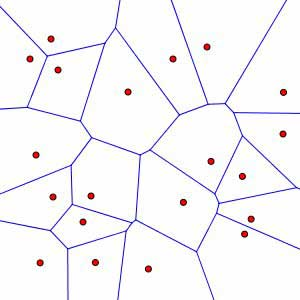
\includegraphics[scale=0.65]{Images/voronoi.jpg}
    \caption{Voronoi Diagram\cite{voronoipic}}
\end{figure}
%--------------------------------------------------------------------------------------
\subsection{Tesselation Generation Algorithms}\label{tes:sec:tga}
%
\subsubsection{Fortunes' Algorithm}\label{tes:ssec:fort}
%
\subsubsection{K-Means Algorithm}\label{tes:ssec:kma}
%--------------------------------------------------------------------------------------